\PassOptionsToPackage{table}{xcolor}
\PassOptionsToPackage{usenames,dvipsnames}{color}

%%%%%%%%%%%%%%%%%%%%%%%%%%%%%%%%%%%%%%%%%%%%%%%%%%%%%%%%%%%%
%%%%%            EXA2CT proto-app -- exaMD             %%%%%
%%%%%%%%%%%%%%%%%%%%%%%%%%%%%%%%%%%%%%%%%%%%%%%%%%%%%%%%%%%%
%%%%%  History:                                        %%%%%
%%%%%   v1.0 - Chris Goodyer, December 2014            %%%%%
%%%%%   v2.0 - Jon Gibson, October 2016                %%%%%
%%%%%%%%%%%%%%%%%%%%%%%%%%%%%%%%%%%%%%%%%%%%%%%%%%%%%%%%%%%%
% ------------------------------------------------------------------------------
% The format is based on: 
%         LaTeX Template: Titlepage
%         This is a title page template which be used for both articles and reports.
%
%         Copyright: http://www.howtotex.com/
%         Date: April 2011
% ------------------------------------------------------------------------------

% -------------------------------------------------------------------------------
% Preamble
% -------------------------------------------------------------------------------
%\documentclass[paper=a4, fontsize=11pt,twoside,bibtotoc]{scrartcl}		% KOMA article
\documentclass[paper=a4, fontsize=11pt,bibtotoc]{scrartcl}		% KOMA article
\usepackage[a4paper,pdftex]{geometry}					% A4paper margins
\oddsidemargin -10mm						% Remove 'twosided' indentation
\topmargin -10mm
\textheight 24.5cm
\textwidth 17.5cm

\parskip 5pt

\usepackage[english]{babel}
%\usepackage[protrusion=true,expansion=true]{microtype}	
\usepackage{amsmath,amsfonts,amsthm,amssymb}
\usepackage{graphicx}

%% Custom sectioning (sectsty package)
\usepackage{sectsty}            % Custom sectioning (see below)

\usepackage[usenames,dvipsnames]{xcolor}

\usepackage{times,mathptmx}

\usepackage{bbding}		% Font for chosen ticks and crosses

\usepackage{graphicx}

\usepackage{authblk}

\usepackage{epstopdf}		% For using eps figures with PDF LaTeX

\usepackage{tocloft}		% For dots in table of contents + \cftsecleader below

\usepackage{algorithm} 		% Algorithms
\usepackage{algorithmic} 	% Algorithms

\usepackage{multicol}		% Multiple columns

\usepackage{tikz}		% Drawing
\usetikzlibrary{patterns}	% Drawing patterns
\usepgflibrary{patterns}	% Drawing patterns

\usepackage{enumerate}		% Modified enumerate environment with sequentially named numbers (See Obj.)

\usepackage{paralist}		% modification of list separation spacing using  {asparaitem}

\usepackage{xstring}		% Adds the \IfEqCase command to use in command definitions

\usepackage[bookmarks,bookmarksnumbered,colorlinks,linkcolor=black,citecolor=blue,urlcolor=black]{hyperref}		% set up indexing of the document when using pdflatex

\allsectionsfont{\centering \normalfont\scshape}        % Change font of al section commands

\usepackage{framed}
\usepackage{bold-extra}
\usepackage{longtable}

\usepackage{enumitem}
\newlist{guide}{enumerate}{10}
\setlist[guide]{label*=\thesection.\arabic*.}
%\setenumerate{leftmargin=3.2em,labelsep=1em}
%\setenumerate[1]{label=\thesection.\arabic*)}
%\setenumerate[2]{label=\thesection.\arabic*.\alph*,topsep=0pt}
%\setenumerate[3]{label=\roman*,topsep=0pt}



% ------------------------------------------------------------------------------
% Definitions (do not change this)
% ------------------------------------------------------------------------------
\newcommand{\HRule}[1]{\rule{\linewidth}{#1}} 	% Horizontal rule

\makeatletter							% Title
\def\printtitle{%						
    {\centering \@title\par}}
\makeatother									

\makeatletter							% Author
\def\printauthor{%					
    {\centering \large \@author}}				
\makeatother							

% ------------------------------------------------------------------------------
% Metadata (Change this)
% ------------------------------------------------------------------------------
\title{ 	% Subtitle of the document
		 	~\mbox{ }\\[1.0cm]									% 1cm spacing
			\HRule{2pt} \\										% Upper rule
			\Huge \textbf{exa\uppercase{MD} User Guide}\\	% Title
		 	~\mbox{ }\\[0.5cm]									% 1cm spacing
			\Large \textbf{A scalable proto-app library for Molecular Dynamics using the Adaptive Midpoint method} % Title
			\HRule{2pt} \\ [0.5cm]									% Lower rule + 0.5cm spacing
			\normalsize %\today									% Todays date
		}
%\title{Calculating interactions for efficient Midpoint M.D. calculations}
%\author{Chris Goodyer}

\author{
		Christopher Goodyer and Jon Gibson\\	
		Numerical Algorithms Group\\
%        \texttt{chris.goodyer@nag.co.uk} \\
}

%\usepackage{scrpage}
\usepackage[automark]{scrpage2} % This should be set AFTER setting up the page geometry
\pagestyle{scrheadings}
% \ohead{\pagemark} 
 \cehead{EXA2CT} 
 \cohead{exaMD -- A scalable proto-app library for M.D.} 
 \ofoot[]{} 
 \cofoot[]{\pagemark} 
 \cefoot[]{\pagemark} 
%\makeatletter
%  \markboth{Left}{Right}
%\makeatother

\lehead{\rightmark}

% ------------------------------------------------------------------------------
% Macros
% ------------------------------------------------------------------------------
%\newenvironment{codebox}{\begin{center}\begin{framed}[0.75\linewidth]\tt}{\end{framed}\end{center}}
%\newenvironment{codebox}{\begin{MakeFramed}{\hsize0.99\linewidth\advance\hsize-\width\FrameRestore}\tt}{\end{MakeFramed}}
\newenvironment{codebox}{\begin{MakeFramed}{\hsize0.8\linewidth\advance\hsize+0pt\FrameRestore}\normalfont\ttfamily}{\end{MakeFramed}}
\newenvironment{filebox}{\begin{center}\begin{MakeFramed}{\hsize0.99\linewidth\advance\hsize-\width\FrameRestore}\normalfont\ttfamily\begin{tabular}{l}}{\end{tabular}\end{MakeFramed}\end{center}}
\newcommand{\prompt}[1]{\textsl{\%} \textbf{#1}}
\newcommand{\exclude}[1]{}


% Macros, environments, etc

%\setcounter{tocdepth}{1}				% For only one level in ToC
\renewcommand{\cftsecleader}{\cftdotfill{\cftdotsep}}	% For dots in table of contents



%%%%%%%%%%%%%%% EPS conversion
\exclude{
\newif\ifpdf
\ifx\pdfoutput\undefined
   \pdffalse
\else
   \pdfoutput=1
   \pdftrue
\fi
\ifpdf
   \usepackage{graphicx}
   \usepackage{epstopdf}
   \DeclareGraphicsRule{.eps}{pdf}{.pdf}{`epstopdf #1}
   \pdfcompresslevel=9
\else
   \usepackage{graphicx}
\fi
}
%%%%%%%%%%%%%%%%%%%%%%%%%%%%%%
%%%%%%%%%% PDF document properties
\hypersetup{
	pdfinfo={
      		Title={EXA2CT proto-app},
          	Subject={EXA2CT work on a Molecular Dynamics Proto-app using the Adaptive Midpoint method},
              	Author={Chris Goodyer, Jon Gibson},
              	Keywords={Parallel, Molecular Dynamics, distributed memory, code optimisation, Midpoint method}
	}
}
                    


% Commands

\newcommand{\TT}[1]{\texttt{#1}}
\newcommand{\Amat}{$\mathbf{A}$}
\newcommand{\Bmat}{$\mathbf{B}$}
\newcommand{\Cmat}{$\mathbf{C}$}
\newcommand{\Umat}{$\mathbf{U}$}
\newcommand{\Smat}{$\mathbf{S}$}
\newcommand{\Vmat}{$\mathbf{V}$}
\newcommand{\code}[1]{\begin{codebox}#1\end{codebox}}
\newcommand{\tab}{~~\mbox{ }~~~}

%\renewcommand{\theenumi}{\thesection.\arabic{enumi}}


%%%%%%%%%%%%%%%%%%%%%%%%%%%%%%%%%%%%%%%%%%%%%%%%%%%%%%%%%%%%%%%%%%%%%%%%%%%%%%%%%%%%%%%%%%%%%%%%%%%%%%%%%%%%%%%%%%%%%%%%%%%%%%%%%%%%%%%%%%%%%%%%%%%%
%%%%%%%%%%%%%%%%%%%%%%%%%%%%%%%%%%%%%%%%%%%%%%%%%%%%%%%%%%%%%%%%%%%%%%%%%%%%%%%%%%%%%%%%%%%%%%%%%%%%%%%%%%%%%%%%%%%%%%%%%%%%%%%%%%%%%%%%%%%%%%%%%%%%
%%%%%%%%%%%%%%%%%%%%%%%%%%%%%%%%%%%%%%%%%%%%%%%%%%%%%%%%%%%%%%%%%%%%%%%%%%%%%%%%%%%%%%%%%%%%%%%%%%%%%%%%%%%%%%%%%%%%%%%%%%%%%%%%%%%%%%%%%%%%%%%%%%%%
% ------------------------------------------------------------------------------
% Begin document
% ------------------------------------------------------------------------------

\begin{document}

% ------------------------------------------------------------------------------
% Maketitle
% ------------------------------------------------------------------------------
\thispagestyle{empty}				% Remove page numbering on this page

\printtitle					% Print the title data as defined above
  	\vfill
\printauthor					% Print the author data as defined above
  	\vfill
\centerline{Version 2.0 -- October 2016}

\newpage

\tableofcontents

\section*{Acknowledgements}

The Adaptive Midpoint method is implemented here, following the original idea and suggestion of Simone Melchionna, 
in order to investigate its potential use for Molecular Dynamics simulations
in the presence of coarse-grained force fields and intrinsically sparse systems, such as occur in macromolecular suspensions
and cellular environments.
Thanks are due to Simone Melchionna and the other developers of the MUPHY simulation software for the base application around which 
this proto-app library has been built and for their assistance and guidance during its development.

\noindent
This code has been developed as part of the European Union's Seventh framework
Programme for research, technological development and demonstration under grant agreement No. 610741.

\noindent
We acknowledge PRACE for awarding us access to resource MareNostrum based in Spain at Barcelona Supercomputing Center and resource Marconi 
based in Italy at Cineca.

\clearpage

%%%%%%%%%%%%%%%%%%%%%%%%%%%%%%%%%%%%%%%%%%%%%%%%%%%%%%%%%%%%%%%%%%%%%%%%%%%%%%%%%%%%%%%%%%%%%%%%%%%%%%%%%%%%%%%%%%%%%%%%%%%%%%%%%%%%%%%%%%%%%%%%%%%%

\section{Overview}

The \TT{exaMD} proto-app parallel library implements the particle interaction calculations of a Molecular Dynamics (MD) code using the Midpoint 
method. An example driver program (\TT{exaMD.f90}) and cost function\\ 
(\TT{lennardjones\_12} in \TT{user\_func.f90}) 
are provided to illustrate the use of the routines. The code is written in Fortran with MPI. 

The Midpoint method is described in Section~\ref{SEC_Midpoint} and its implementation in \TT{exaMD} in Section~\ref{SEC_Imp}.
Instructions on building and using the library are given in Section~\ref{SEC_Compile}.
Testing has been done up to 6,000 cores and good results achieved for cases with sufficient computational work.  
The performance is discussed in Section~\ref{SEC_Results}. 

%%%%%%%%%%%%%%%%%%%%%%%%%%%%%%%%%%%%%%%%%%%%%%%%%%%%%%%%%%%%%%%%%%%%%%%%%%%%%%%%%%%%%%%%%%%%%%%%%%%%%%%%%%%%%%%%%%%%%%%%%%%%%%%%%%%%%%%%%%%%%%%%%%%%

\section{The Adaptive Midpoint method} \label{SEC_Midpoint}

Generally, in Molecular Dynamics the forces are calculated between all pairs of particles with a separation less than a given cutoff distance, 
$R_c$. 
Recently, new methods have been devised in order to optimize the search volume for particle interactions. These include the Tower-Plate method~\cite{Larson08} 
and the Midpoint method~\cite{Bowers06}, the latter having been extended in an adaptive sense in~\cite{FSSM17}. 

In the conventional Midpoint method, the domain is split into blocks of side $R_c/2$ so that distances 
and interactions need only be considered between neighbouring blocks. Subsequently, a search radius of $R_c/2$ is considered around every home 
block so that particles within a 
distance of $R_c$ from each other can be found by searching from a point somewhere between the two. 
Force calculations are performed on the process that owns this midpoint block. The advantage of this method is that the search volume is $\frac{4}{3}\pi{(\frac{R_c}{2})}^3$ rather than 
$\frac{4}{3}\pi{R_c}^3$, a reduction by a factor of eight. This means that, on average, eight times fewer particle pairings need to be considered.  
This is balanced against sometimes needing to send more messages post-calculation, given that both particles in a calculation on one process may 
live on other processes.

When parallelised, with each process owning a subset of blocks, this method typically means that 
each process exchanges particle information with those processes responsible for the neighbouring domains. By considering the order in which 
interactions between particles in different blocks are calculated, it is possible to ensure that each interaction is only calculated once. Each 
block would only have to consider a subset of its neighbours, although if the blocks are on different processes then the result would have to be 
communicated to the one that doesn't perform the calculation. 

The conventional Midpoint method is suboptimal when applied to sparse molecular systems, such as occur in coarse-grained 
Molecular Dynamics simulations, because sparsity causes an imbalance in the communication that impacts negatively on the parallel performance. 
The Adaptive Midpoint method specifically targets these situations by providing a dynamic and general way to determine the best communication 
pattern as molecules move in time ~\cite{FSSM17}.
The key idea is to perform an on-the-fly recalculation of the communication pattern as molecules move away from a starting position. 
Given the large difference in timescales between the fast local motion of atoms and the diffusive displacement of molecules as a whole, 
re-partitioning can be done sporadically as timestepping advances, thus taking only a negligible fraction of the total 
computing time (further details are found in ~\cite{FSSM17}).


In our approach, the domain is divided into cubic blocks of width $R_c/2$ and then the blocks are partitioned 
amongst the processes. Typically, a process would have many blocks and would communicate with a number of other processes.
Figure~\ref{FIG_Homeblock} shows the set of neighbouring blocks for both two and three dimensions, with the home block being number 5 in each case.
\begin{figure}
	\centerline{
		\raisebox{-0.5\height}{
			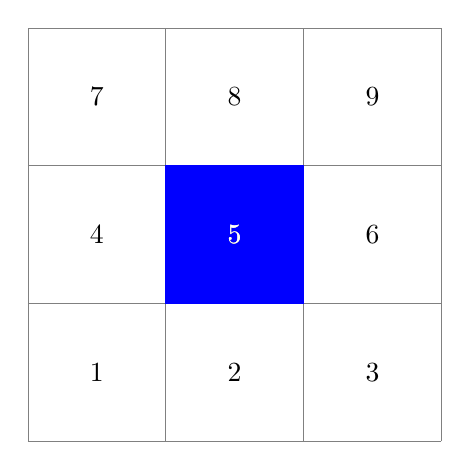
\begin{tikzpicture}[scale=1.75]
				\draw[help lines] (0,0) grid (3,3);
				\draw[blue, fill=blue] (1,1) rectangle (2,2);
				\foreach \p in {0,1,2} {
					\foreach \q [evaluate={\x=int(3*\p+\q)}] in {1,2,3} {
						\node at (\q-0.5,\p+0.5) {\x};
					}
					\node[white] at (1.5,1.5) {5};
				}
			\end{tikzpicture}
		}
		\hspace{0.5cm}
		\raisebox{-0.5\height}{
			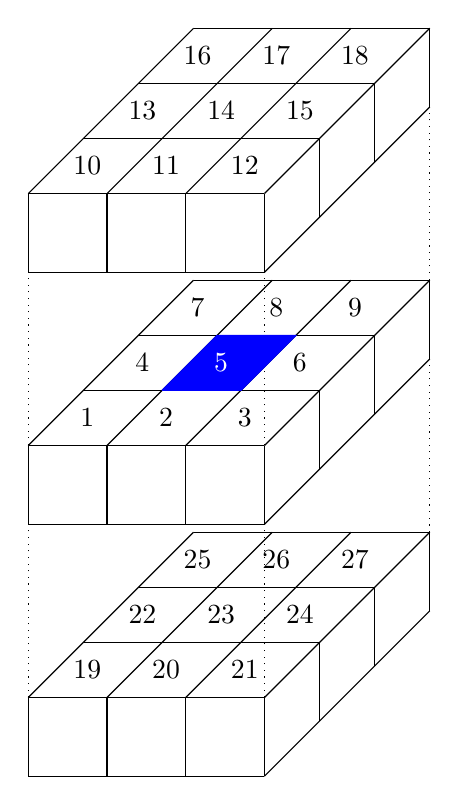
\begin{tikzpicture}
				\foreach \l in {0,1,2} {
					\draw (0,0+\l*3.2) -- (3,0+\l*3.2) ;
					\draw (3,0+\l*3.2) -- (3+3*0.7,3*0.7+\l*3.2) ;
					\foreach \p in {0,1,2,3} {
						\draw (\p,0+\l*3.2) -- (\p,1+\l*3.2) ;
						\draw (0+\p*0.7,1+\p*0.7+\l*3.2) -- (3+\p*0.7,1+\p*0.7+\l*3.2) ;
						\draw (\p,1+\l*3.2) -- (\p+3*0.7,1+3*0.7+\l*3.2) ;
						\draw (3+\p*0.7,\p*0.7+\l*3.2) -- (3+\p*0.7,1+\p*0.7+\l*3.2) ;
					}
				}
				\foreach \p in {0,1,2} {
					\foreach \q [evaluate={\x=int(3*\p+\q)}] in {1,2,3} {
						\node at (\q-0.25+0.7*\p,\p*0.7+0.5+3.2+0.85) {\x};
					}
					\foreach \q [evaluate={\x=int(3*\p+\q+9)}] in {1,2,3} {
						\node at (\q-0.25+0.7*\p,\p*0.7+0.5+3.2+0.85+3.2) {\x};
					}
					\foreach \q [evaluate={\x=int(3*\p+\q+18)}] in {1,2,3} {
						\node at (\q-0.25+0.7*\p,\p*0.7+0.5+3.2+0.85-3.2) {\x};
					}
				}
				\draw[dotted] (0,1) -- (0,2*3.2); 
				\draw[dotted] (3,1) -- (3,2*3.2); 
				\draw[dotted] (3+3*0.7,1+3*0.7) -- (3+3*0.7,1+3*0.7+2*3.2); 
				\draw[blue, fill=blue] (1.7,1.7+3.2) -- (2.7,1.7+3.2) -- (3.4,2.4+3.2) -- (2.4,2.4+3.2) -- (1.7,1.7+3.2);
				\node[white] at (2-0.25+0.7,0.7+0.5+3.2+0.85) {5};
			\end{tikzpicture}
		}
	}
	\caption{Schematic showing neighbouring blocks in (a) 2D and (b) 3D}
	\label{FIG_Homeblock}
\end{figure}
Obviously, two particles in the same block would also have their midpoint in the block. However, when the particles are in different blocks (and so 
potentially also different processes), a calculation may be required to determine in which block the midpoint lies. In order to avoid this, a set of 
rules can be defined which specify which block will own a particular calculation. For the simpler 2D example, these rules are shown in 
Table~\ref{TAB_interact2d}. Note the following points.
\newcommand{\NO}[1]{
	\IfEqCase{#1}{
		{0}{\color{white}} % 1 <-> 9
		{1}{\color{Mulberry}} % 1 <-> 9
		{2}{\color{CornflowerBlue}} % 2 <-> 9
		{3}{\color{Mahogany}} % 2 <-> 8
		{4}{\color{YellowGreen}} % 4 <-> 9
		{5}{\color{blue}} % 5 <-> 5
		{6}{\color{red}} % 5 <-> 6
		{7}{\color{OliveGreen}} % 5 <-> 7 
		{8}{\color{Rhodamine}} % 5 <-> 8
		{9}{\color{RoyalPurple}} % 5 <-> 9
		{10}{\color{YellowOrange}} % 4 <-> 6
		{11}{\color{Goldenrod}} % 3 <-> 7
		{12}{\color{JungleGreen}} % 3 <-> 8
		{13}{\color{MidnightBlue}} % 6 <-> 7
	}
	\XSolidBrush
}
\newcommand{\YES}[1]{
	\IfEqCase{#1}{
		{0}{\cellcolor{black}\color{white}} % 1 <-> 9
		{1}{\cellcolor{Mulberry}\color{white}} % 1 <-> 9
		{2}{\cellcolor{CornflowerBlue}\color{white}} % 2 <-> 9
		{3}{\cellcolor{Mahogany}\color{white}} % 2 <-> 8
		{4}{\cellcolor{YellowGreen}\color{white}} % 4 <-> 9
		{5}{\cellcolor{blue}\color{white}} % 5 <-> 5
		{6}{\cellcolor{red}\color{white}} % 5 <-> 6
		{7}{\cellcolor{OliveGreen}\color{white}} % 5 <-> 7 
		{8}{\cellcolor{Rhodamine}\color{white}} % 5 <-> 8
		{9}{\cellcolor{RoyalPurple}\color{white}} % 5 <-> 9
		{10}{\cellcolor{YellowOrange}\color{white}} % 4 <-> 6
		{11}{\cellcolor{Goldenrod}\color{white}} % 3 <-> 7
		{12}{\cellcolor{JungleGreen}\color{white}} % 3 <-> 8
		{13}{\cellcolor{MidnightBlue}\color{white}} % 6 <-> 7
	}
	\Checkmark
}
\newcommand{\pair}[2]{$#1$$\leftrightarrow$$#2$}
\begin{table}
	\centering
	\renewcommand{\arraystretch}{1.5}
	\begin{tabular}{|c|*{9}{c|}}
		\hline
		Particle two& \multicolumn{9}{c|}{Particle one}\\
		& 	1 &	2 &	3 &	4 &	5 &	6 & 	7 &	8 &	9 \\	
		\hline
		1&\NO{5} &\NO{6} &\NO{10}&\NO{8} &\NO{9} &\NO{4} &\NO{3} &\NO{2} &\YES{1} \\	
		2&	 &\NO{5} &\NO{6} &\NO{7} &\NO{8} &\NO{9} &\NO{12}&\YES{3}&\YES{2} \\	
		3&	 &	 &\NO{5} &\NO{13}&\NO{7} &\NO{8} &\YES{11}&\YES{12}&\NO{3} \\	
		4&	 &	 &	 &\NO{5} &\NO{6} &\YES{10}&\NO{8} &\NO{9} &\YES{4} \\	
		5&	 &	 &	 &	 &\YES{5}&\YES{6}&\YES{7}&\YES{8}&\YES{9} \\	
		6&	 &	 &	 &	 &	 &\NO{5} &\YES{13}&\NO{7} &\NO{8} \\	
		7&	 &	 &	 &	 &	 &	 &\NO{5} &\NO{6} &\NO{4} \\	
		8&	 &	 &	 &	 &	 &	 & 	 &\NO{5} &\NO{6} \\	
		9&	 &	 &	 &	 &	 &	 & 	 &	 &\NO{5} \\	
		\hline
	\end{tabular}
	\caption{Midpoint interactions in 2D. The same colour indicates equivalent operations.}
	\label{TAB_interact2d}
\end{table}

\begin{itemize}
	\item{The main diagonal shows interactions between particles in the same block. These will only be evaluated on the home block, hence (5,5) 
              is the only tick. All the colours along this diagonal are blue to indicate that they are all equivalent operations.}
	\item{The interactions below the main diagonal need not be evaluated, given the symmetry. Avoiding the repetition of calculations within a 
              given block must also be considered.} 
	\item{For particles in the home block (5), the only interactions to consider are those with the three blocks above (7, 8 and 9) and the one 
	      to the right (6). The interactions with the other four blocks will be calculated while those blocks are the home block. For example, 
              the interaction \pair{4}{5} is evaluated as \pair{5}{6} when the home block is one to the left. 
	      This neighbouring relationship is replicated in the pairings \pair{1}{2}, \pair{2}{3}, \pair{7}{8} and \pair{8}{9}.  The 
	      colouring on the table is thus a red ticked cell at (5,6), with red crosses at (1,2), (2,3), (4,5), (7,8) and (8,9).} 
	\item{Other equivalent pairs are similarly coloured to highlight which pairs need to be calculated on the home block.} 
	\item{In total there are 13 pairs of blocks which require their interactions to be calculated on the home block, out of a possible 45.} 
\end{itemize}

When considering the 3D problem, also shown in Figure~\ref{FIG_Homeblock}, there are obviously many more combinations of blocks to consider, although 
the principles are the same. The interactions that need calculating on any given home block are shown in Table~\ref{TAB_interact3d}.
The table shows that only 63 pairs need to be considered out of a total of 378 potential interactions.
\renewcommand{\NO}[1]{
	\IfEqCase{#1}{
		{0}{\cellcolor{white}\color{white}} % 
		{1}{} {2}{} {3}{} {4}{} {5}{} {6}{} {7}{} {8}{} {9}{} {10}{} {11}{} {12}{} {13}{}
	}
	\XSolidBrush
}
\renewcommand{\YES}[1]{\cellcolor{black}\color{white}\Checkmark}
\begin{table}        	
	\centering
	\scriptsize
	%\tiny
	%\renewcommand{\arraystretch}{1.5}
	\begin{tabular}{|c|*{27}{>{\hspace{-4pt}}c<{\hspace{-4pt}}|}}
		\hline
		P2& \multicolumn{27}{c|}{Particle one}\\
		& 	1 &	2 &	3 &	4 &	5 &	6 & 	7 &	8 &	9 
		& 	10 &	11 &	12 &	13 &	14 &	15 &	16 & 	17 &	18
		& 	19 &	20 &	21 &	22 &	23 &	24 &	25 &	26 & 	27
		\\	
		\hline
		1&\NO{5} &\NO{6} &\NO{10}&\NO{8} &\NO{9} &\NO{4} &\NO{3} &\NO{2} &\YES{1}
		&\NO{8} &\NO{9} &\NO{4}&\NO{9} &\NO{13} &\NO{12} &\NO{11} &\NO{10} &\YES{0}
		&\NO{1} &\NO{1} &\NO{1}&\NO{1} &\NO{1} &\NO{1} &\NO{1} &\NO{1} &\NO{1}
		 \\	
		2&	 &\NO{5} &\NO{6} &\NO{7} &\NO{8} &\NO{9} &\NO{12}&\YES{3}&\YES{2} 
		&\NO{7} &\NO{8} &\NO{9}&\NO{12} &\NO{9} &\NO{13} &\YES{10} &\YES{11} &\YES{10}
		&\NO{1} &\NO{1} &\NO{1}&\NO{1} &\NO{1} &\NO{1} &\NO{1} &\NO{1} &\NO{1}
		\\	
		3&	 &	 &\NO{5} &\NO{13}&\NO{7} &\NO{8} &\YES{11}&\YES{12}&\NO{3} 
		&\NO{13} &\NO{7} &\NO{8}&\NO{4} &\NO{12} &\NO{9} &\YES{0} &\NO{10} &\NO{11}
		&\NO{1} &\NO{1} &\NO{1}&\NO{1} &\NO{1} &\NO{1} &\NO{1} &\NO{1} &\NO{1}
		\\	
		4&	 &	 &	 &\NO{5} &\NO{6} &\YES{10}&\NO{8} &\NO{9} &\YES{4} 
		&\NO{7} &\NO{11} &\NO{6}&\NO{8} &\NO{9} &\YES{4} &\NO{9} &\NO{13} &\YES{12}
		&\NO{1} &\NO{1} &\NO{1}&\NO{1} &\NO{1} &\NO{1} &\NO{1} &\NO{1} &\NO{1}
		\\	
		5&	 &	 &	 &	 &\YES{5}&\YES{6}&\YES{7}&\YES{8}&\YES{9} 		
		&\YES{10} &\YES{7} &\YES{11}&\YES{7} &\YES{8} &\YES{9} &\YES{12} &\YES{9} &\YES{13}
		&\NO{13} &\NO{9} &\NO{12}&\NO{9} &\NO{8} &\NO{7} &\NO{11} &\NO{7} &\NO{10}
		\\	
		6&	 &	 &	 &	 &	 &\NO{5} &\YES{13}&\NO{7} &\NO{8} 
		&\YES{5} &\NO{10} &\NO{7}&\YES{13} &\NO{7} &\NO{8} &\YES{4} &\NO{12} &\NO{9}
		&\NO{1} &\NO{1} &\NO{1}&\NO{1} &\NO{1} &\NO{1} &\NO{1} &\NO{1} &\NO{1}
		\\	
		7&	 &	 &	 &	 &	 &	 &\NO{5} &\NO{6} &\NO{4} 
		&\NO{2} &\NO{3} &\YES{0}&\NO{7} &\NO{11} &\YES{7} &\NO{8} &\NO{9} &\NO{4}
		&\NO{1} &\NO{1} &\NO{1}&\NO{1} &\NO{1} &\NO{1} &\NO{1} &\NO{1} &\NO{1}
		\\	
		8&	 &	 &	 &	 &	 &	 & 	 &\NO{5} &\NO{6} 
		&\YES{1} &\YES{2} &\YES{3}&\NO{10} &\NO{7} &\NO{11} &\NO{7} &\NO{8} &\NO{9}
		&\NO{1} &\NO{1} &\NO{1}&\NO{1} &\NO{1} &\NO{1} &\NO{1} &\NO{1} &\NO{1}
		\\	
		9&	 &	 &	 &	 &	 &	 & 	 &	 &\NO{5} 
		&\YES{0} &\NO{1} &\NO{2}&\NO{5} &\NO{10} &\NO{7} &\NO{13} &\NO{7} &\NO{8}
		&\NO{1} &\NO{1} &\NO{1}&\NO{1} &\NO{1} &\NO{1} &\NO{1} &\NO{1} &\NO{1}
		\\	
 		10&       &       &       &       &       &       &       &       &
		&\NO{5} &\NO{6} &\NO{10}&\NO{8} &\NO{9} &\NO{4} &\NO{3} &\NO{2} &\NO{1} 
		&\NO{5} &\NO{4} &\NO{10}&\NO{2} &\YES{1} &\NO{11} &\NO{12} &\NO{13} &\YES{0}
		\\	
		11&       &       &       &       &       &       &       &       &
		&	 &\NO{5} &\NO{6} &\NO{7} &\NO{8} &\NO{9} &\NO{12}&\NO{3}&\NO{2}
		&\NO{6} &\NO{5} &\NO{4}&\NO{3} &\YES{2} &\NO{1} &\YES{13} &\YES{12} &\YES{13}
		\\	
		12&       &       &       &       &       &       &       &       &
			&	 &	 &\NO{5} &\NO{13}&\NO{7} &\NO{8} &\NO{11}&\NO{12}&\NO{3}
		&\NO{9} &\NO{6} &\NO{5}&\NO{7} &\YES{3} &\NO{2} &\YES{0} &\NO{13} &\NO{12}
		\\	
		13&       &       &       &       &       &       &       &       &
		&	 &	 &	 &\NO{5} &\NO{6} &\NO{10}&\NO{8} &\NO{9} &\NO{4}
		&\NO{8} &\NO{7} &\NO{1}&\NO{5} &\YES{4} &\YES{10} &\NO{2} &\NO{1} &\YES{11}
		\\	
		14&       &       &       &       &       &       &       &       &
		&	 &	 &	 &	 &\NO{5}&\NO{6}&\NO{7}&\NO{8}&\NO{9}
		&\NO{9} &\NO{8} &\NO{7}&\NO{6} &\YES{5} &\NO{4} &\NO{3} &\NO{2} &\NO{1}
		\\	
		15&       &       &       &       &       &       &       &       &
		&	 &	 &	 &	 &	 &\NO{5} &\NO{13}&\NO{7} &\NO{8} 
		&\NO{2} &\NO{9} &\NO{8}&\YES{9} &\YES{6} &\NO{5} &\YES{7} &\NO{3} &\NO{2}
		\\	
		16&       &       &       &       &       &       &       &       &
		&	 &	 &	 &	 &	 &	 &\NO{5} &\NO{6} &\NO{4} 
		&\NO{3} &\NO{4} &\YES{0}&\NO{8} &\YES{7} &\YES{1} &\NO{5} &\NO{4} &\NO{10}
		\\	
		17&       &       &       &       &       &       &       &       &
		&	 &	 &	 &	 &	 &	 &	 &\NO{5} &\NO{6} 
		&\NO{5} &\YES{3} &\YES{4}&\NO{9} &\YES{8} &\NO{7} &\NO{6} &\NO{5} &\NO{4}
		\\	
		18&       &       &       &       &       &       &       &       &
		&	 &	 &	 &	 &	 &	 &	 &	 &\NO{5}
		&\YES{0} &\YES{5} &\NO{3}&\YES{2} &\YES{9} &\NO{8} &\NO{9} &\NO{6} &\NO{5}
		\\	
		19&       &       &       &       &       &       &       &       &
		&       &       &       &       &       &       &       &       &
		&\NO{5} &\NO{6} &\NO{10}&\NO{8} &\NO{9} &\NO{4} &\NO{3} &\NO{2} &\NO{1}
		\\	
		20&       &       &       &       &       &       &       &       &
		&       &       &       &       &       &       &       &       &
		&	 &\NO{5} &\NO{6} &\NO{7} &\NO{8} &\NO{9} &\NO{12}&\NO{3}&\NO{2} 
		\\	
		21&       &       &       &       &       &       &       &       &
		&       &       &       &       &       &       &       &       &
		&	 &	 &\NO{5} &\NO{13}&\NO{7} &\NO{8} &\NO{11}&\NO{12}&\NO{3} 
		\\	
		22&       &       &       &       &       &       &       &       &
		&       &       &       &       &       &       &       &       &
		&	 &	 &	 &\NO{5} &\NO{6} &\NO{10}&\NO{8} &\NO{9} &\NO{4} 
		\\	
		23&       &       &       &       &       &       &       &       &
		&       &       &       &       &       &       &       &       &
		&	 &	 &	 &	 &\NO{5}&\NO{6}&\NO{7}&\NO{8}&\NO{9}
		\\	
		24&       &       &       &       &       &       &       &       &
		&       &       &       &       &       &       &       &       &
		&	 &	 &	 &	 &	 &\NO{5} &\NO{13}&\NO{7} &\NO{8}
		\\	
		25&       &       &       &       &       &       &       &       &
		&       &       &       &       &       &       &       &       &
		&	 &	 &	 &	 &	 &	 &\NO{5} &\NO{6} &\NO{4} 
		\\	
		26&       &       &       &       &       &       &       &       &
		&       &       &       &       &       &       &       &       &
		&	 &	 &	 &	 &	 &	 &	 &\NO{5} &\NO{6}
		\\	
		27&       &       &       &       &       &       &       &       &
		&       &       &       &       &       &       &       &       &
		&	 &	 &	 &	 &	 &	 &	 &	 &\NO{5}
		\\	
		\hline
	\end{tabular}
	\caption{Midpoint interactions in 3D}
	\label{TAB_interact3d}
\end{table}

%%%%%%%%%%%%%%%%%%%%%%%%%%%%%%%%%%%%%%%%%%%%%%%%%%%%%%%%%%%%%%%%%%%%%%%%%%%%%%%%%%%%%%%%%%%%%%%%%%%%%%%%%%%%%%%%%%%%%%%%%%%%%%%%%%%%%%%%%%%%%%%%%%%%

\section{Implementation}\label{SEC_Imp}

Algorithm~\ref{ALG_midpoint} shows how a single force calculation step of the midpoint method has been implemented in the exaMD proto-app library. 
The first three steps of the algorithm are described in Section~\ref{SEC_Partitioning}, domain decomposition and partitioning, with the remainder in 
the following section on the midpoint algorithm, which also includes a description of the overlap variant of the algorithm. 
Section~\ref{SEC_MPI} then describes the MPI communication within the code. 
\begin{algorithm}[tbp]
	\begin{algorithmic}[1]
		\STATE{Decompose the domain into \emph{blocks} (cubes of side length $R_c/2$).}\label{LINE_decompose}
		\STATE{Generate the particle distribution (either randomly or read from file).}\label{LINE_generate}
		\STATE{Partition the domain between processes, i.e. map blocks to processes. }\label{LINE_partition}
		\STATE{Initiate sending of particle positions to processes with neighbouring blocks using non-blocking 
                       communication.}\label{LINE_sendP}
		\FOR{$block_{interior}$ = 1 to $n_{interior}$}\label{LINE_mainloopstart}
			\IF{$block_{interior}$ = a multiple of 10\% of $n_{interior}$ \AND all messages have newly arrived}\label{LINE_recvP}
				\FOR{$block_{boundary}$ = 1 to $n_{boundary}$}
					\FOR{permutation\_index = 1 to 63}
						\STATE{b1=permutation(permutation\_index,1)}
						\STATE{b2=permutation(permutation\_index,2)}
						\STATE{Compute interaction(b1,b2)}
					\ENDFOR
				\ENDFOR
				\STATE{Send forces back to neighbours using non-blocking communication.}\label{LINE_sendF}
			\ENDIF
			\FOR{permutation\_index  = 1 to 63}\label{LINE_intloop}
				\STATE{b1=permutation(permutation\_index,1)}
				\STATE{b2=permutation(permutation\_index,2)}
				\STATE{Compute interaction(b1,b2)}
			\ENDFOR\label{LINE_intloopend}
		\ENDFOR\label{LINE_mainloopend}
		\STATE{Complete receiving of forces.}\label{LINE_recvforces}
	\end{algorithmic}
	\caption{Pseudo-code showing how non-blocking communication allows overlap of computation and communication in a 
		 single force calculation step of the midpoint method.}
	\label{ALG_midpoint}
\end{algorithm}


\subsection{Domain Decomposition and Partitioning} \label{SEC_Partitioning}

In the first step of Algorithm~\ref{ALG_midpoint}, the global box is divided up into blocks of size 
$\frac{R_c}{2}\times\frac{R_c}{2}\times\frac{R_c}{2}$, with the three faces at the greatest distance from the origin having larger blocks, 
to match the global box boundary. If the global box is cubic with a side of length $L$ and the block length is $d=R_c/2$, 
then there will be $\mathrm{int}\left(\frac{L}{d}\right)$ blocks along each side of the box and the total number of blocks will be
\begin{equation}
	n_b = \left[\mathrm{int}\left(\frac{L}{d}\right)\right]^3 \nonumber
\end{equation} 
Along each side there will be
\begin{eqnarray}
	\mathrm{int}\left(\frac{L}{d}\right) -1 &\mathrm{blocks~of~width}& d \nonumber \\
	\mathrm{and~1} &\mathrm{block~of~width}& L -d\left[\mathrm{int}\left(\frac{L}{d}\right) - 1 \right] \nonumber
\end{eqnarray}

The list of particles is then created, either by randomly generating positions within the global domain or by reading a previously-generated 
distribution from file. The particles are subject to the constraint that 
they must be a distance of at least 1.0 from all other particles, including over the periodic boundaries. This imposes an upper limit on the number 
of particles that can be placed in a domain of a given size. As each particle is generated, the block in which it is located is determined. 

To help facilitate arbitrary process counts and high quality partitions, the package METIS~\cite{Karypis06} is used to partition the blocks 
amongst the processes (step~\ref{LINE_partition} of Algorithm~\ref{ALG_midpoint}). METIS is software that performs graph partitioning based
on multilevel recursive-bisection that is particularly efficient for sparse matrices. It creates contiguous partitions with minimal 
communication costs between neighbouring processes. In a full 
production code, ParMETIS~\cite{Karypis02} could be used instead to perform the partitioning in parallel. Alternatively, another partitioner could 
be used. The routine \TT{exaMD\_partition\_domain} in \TT{exaMD\_partitioning.f90} could be adapted to call another partitioner or use a 
previously set-up partition. Regardless of which method is used, after partitioning all processes need to call \TT{exaMD\_setup\_partitioned\_grid} to 
set up the correct data structures.


\subsection{The Midpoint Algorithm and Adaptivity}

The code employs a number of look-up tables. Table~\ref{TAB_Interactions} shows the ``permutation list'', extracted from the interactions shown in 
Table~\ref{TAB_interact3d}. 
\begin{table}
	\centering
	\begin{tabular}{|*{10}{c}|}
		\hline 
		\pair{5}{5}	& \pair{5}{6}	& \pair{5}{7}	& \pair{5}{8}	& \pair{5}{9}	& 
                \pair{5}{10}	& \pair{5}{11}	& \pair{5}{12}	& \pair{5}{13}	& \pair{5}{14}	\\ 
                \pair{5}{15}	& \pair{5}{16}	& \pair{5}{17}	& \pair{5}{18}	& \pair{4}{6}	& 
		\pair{4}{9}	& \pair{4}{15}	& \pair{4}{18}	& \pair{6}{7}	& \pair{6}{10}	\\ 
                \pair{6}{13}	& \pair{6}{16}	& \pair{3}{7}	& \pair{3}{8}	& \pair{3}{16}	& 
                \pair{2}{8}	& \pair{2}{9}	& \pair{2}{16}	& \pair{2}{17}	& \pair{2}{18}	\\ 
                \pair{1}{9}	& \pair{1}{18}	& \pair{7}{12}	& \pair{7}{15}	& \pair{8}{10}	& 
                \pair{8}{11}	& \pair{8}{12}	& \pair{9}{10}	& \pair{10}{23}	& \pair{10}{27}	\\ 
                \pair{11}{23}	& \pair{11}{25}	& \pair{11}{26}	& \pair{11}{27}	& \pair{12}{23}	& 
                \pair{12}{25}	& \pair{13}{23}	& \pair{13}{24}	& \pair{13}{27}	& \pair{14}{23}	\\ 
                \pair{15}{22}	& \pair{15}{23}	& \pair{15}{25}	& \pair{16}{21}	& \pair{16}{23}	& 
		\pair{16}{24}	& \pair{17}{20}	& \pair{17}{21}	& \pair{17}{23}	& \pair{18}{19}	\\ 
                \pair{18}{20}	& \pair{18}{22}	& \pair{18}{23}	&&&&&&&\\ 
		\hline 
	\end{tabular} 
	\caption{Block interactions that need calculating in 3D} 
	\label{TAB_Interactions} 
\end{table} 
Lists are also built up of the blocks owned by each process. These are subdivided into lists of \textsl{interior blocks} 
(i.e. with no neighbouring blocks on other processes), lists of \textsl{boundary blocks} (i.e. with at least one of its 26 neighbours on a different 
process) and lists of \textsl{exterior blocks} (i.e. blocks that need to be received from a neighbouring process). These are illustrated in 
Figure~\ref{FIG_blocklists}, where the solid black lines denote process boundaries.
\begin{figure}
	\centering
	\raisebox{-0.5\height}{
		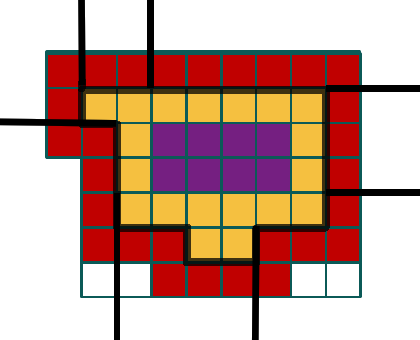
\includegraphics[width=0.5\textwidth]{FIGS/lists_new}
	}
	\raisebox{-0.5\height}{
		\begin{tabular}{l}
			{\color{Purple} \rule{2ex}{2ex} Interior blocks}\\
			{\color{Orange} \rule{2ex}{2ex} Boundary blocks}\\
			{\color{Red} \rule{2ex}{2ex} Exterior blocks}
		\end{tabular}
	}
	\caption{The different types of blocks on a process}
	\label{FIG_blocklists}
\end{figure}
Individual blocks also have a list of the processes they need to communicate with.

With a view to writing efficient parallel code on large process counts, computation and communication were overlapped. This is achieved 
by initiating the sending of the positions (line~\ref{LINE_sendP} of Algorithm~\ref{ALG_midpoint}) before computing any interactions.  
Using the lists of block types, the code then computes the interactions of the interior blocks until all exterior blocks have been received. 
At this point, line~\ref{LINE_recvP} in Algorithm~\ref{ALG_midpoint}, all interactions for the boundary blocks can be calculated. 
Once these boundary blocks are computed, the relevant force information is sent back to the neighbouring processes (line~\ref{LINE_sendF}) before 
completing the calculations on the interior blocks (lines~\ref{LINE_intloop}-\ref{LINE_intloopend}).

The adaptive nature of the Midpoint method leverages the high quality partitioning created by METIS (or by other equivalent, graph-based
partitioning methods), in order to perform on-the-fly recalculation of the communication pattern as molecules move away from their starting positions. 
The user can modify the basic scheme presented in \TT{exaMD.f90} in order to call METIS at regular intervals.

\subsubsection{The Overlap Variant}\label{SEC_overlap}

The overlap variant processes a given boundary block as soon as the messages that block requires have been received, rather than waiting for all 
that process's incoming messages to have been received and then processing all the boundary blocks. The intention is to increase the degree of 
overlap between computation and communication. This alternative approach is shown in Algorithm~\ref{ALG_overlap} (note that only 
lines~\ref{LINE_overlap_diff1} and~\ref{LINE_overlap_diff2} have changed from Algorithm~\ref{ALG_midpoint} but showing the other lines makes it 
easier to understand).
\begin{algorithm}[tbp]
	\begin{algorithmic}[1]
\setcounter{ALC@line}{3}
		\STATE{Initiate sending of particle positions to processes with neighbouring blocks using non-blocking 
                       communication.}
		\FOR{$block_{interior}$ = 1 to $n_{interior}$}\label{LINE_overlap_mainloopstart}
			\IF{$block_{interior}$ = a multiple of 10\% of $n_{interior}$ \AND some messages have newly arrived}\label{LINE_overlap_diff1}
				\FOR{$block_{boundary}$ = 1 to $n_{boundary\_newly\_arrived\_messages}$}\label{LINE_overlap_diff2}
					\FOR{permutation\_index = 1 to 63}
						\STATE{b1=permutation(permutation\_index,1)}
						\STATE{b2=permutation(permutation\_index,2)}
						\STATE{Compute interaction(b1,b2)}
					\ENDFOR
				\ENDFOR
				\STATE{Send forces back to neighbours using non-blocking communication.}
			\ENDIF
			\FOR{permutation\_index  = 1 to 63}
				\STATE{b1=permutation(permutation\_index,1)}
				\STATE{b2=permutation(permutation\_index,2)}
				\STATE{Compute interaction(b1,b2)}
			\ENDFOR
		\ENDFOR \label{LINE_overlap_mainloopend}
		\STATE{Complete receiving of forces.}
	\end{algorithmic}
	\caption{Pseudo-code for the overlap variant of the midpoint method implementation.}
	\label{ALG_overlap}
\end{algorithm}


\subsection{MPI Communication}\label{SEC_MPI}

The code's MPI communication is made up of four distinct phases.
\begin{itemize}
	\item{After the initial distribution of the particles has been calculated, process 0 broadcasts the initial particle counts on every block 
              to all processes. It then sends to each process all the particle positions for the blocks that process owns.}
	\item{At the start of the calculation phase, each process sends to the processes owning its exterior blocks, arrays of any particles 
              positions that they require. They will then receive the particle positions required from the relevant processes. Note that it may be 
              necessary to send data from the same block to multiple processes.}
 	\item{At the end of the calculation phase, the forces calculated for particles in exterior blocks need communicating back to their owning 
              processes. These forces then need adding to both the forces calculated locally and those from other processes.}
	\item{After the forces have been calculated, a global sum of their values and the square of their values is calculated to help verify the 
              results. This is done using calls to \texttt{MPI\_Reduce}.}
\end{itemize}
An important design decision was to locally gather all information being sent to a particular process so that it could be sent in a single message.  
This packing and unpacking may make the code slightly more complicated but the latency of multiple messages could become a significant overhead 
otherwise. 

%%%%%%%%%%%%%%%%%%%%%%%%%%%%%%%%%%%%%%%%%%%%%%%%%%%%%%%%%%%%%%%%%%%%%%%%%%%%%%%%%%%%%%%%%%%%%%%%%%%%%%%%%%%%%%%%%%%%%%%%%%%%%%%%%%%%%%%%%%%%%%%%%%%%

\section{Installation and Usage}\label{SEC_Compile}

\subsection{Building the Proto-app}

The file \TT{exaMD/make.inc} is included by Makefiles in the \TT{exaMD} and \TT{exaMD/SRC} directories and should be the only file you need to edit. 
Set the variable \TT{F90} in \TT{make.inc} to point to your MPI Fortran compiler and \TT{FLAGS} to the appropriate compiler flags. 
By default, the partitioner used is METIS. If this is not currently installed on your system, it can be downloaded from\\
\TT{http://glaros.dtc.umn.edu/gkhome/metis/metis/download}. The variable \TT{METIS\_DIR} in\\ 
\TT{make.inc} needs to be set to your top-level METIS directory.

To compile, simply run 
\begin{codebox}
        \prompt{make}
\end{codebox}
\noindent
from the \TT{exaMD} directory. This will create both an executable, \TT{exaMD}, and a library, \TT{LIB/libexaMD.a}.

If you want to compile the library and not the executable, then run 
\begin{codebox}
        \prompt{make lib}
\end{codebox}

\noindent
To remove all object and module files, the library and executable, run 
\begin{codebox}
        \prompt{make clean}
\end{codebox}


\subsection{Running the Proto-app Driver}

The application should be run using the standard method for running MPI jobs on your system. For example, if this is using \TT{mpirun}, then to 
launch a 16 process job you would use
\begin{codebox}
        \prompt{mpirun -np 16 ./exaMD}
\end{codebox}

\noindent
There are a number of flags that can be given to \TT{exaMD}:

\begin{tabular}{cl}
	\TT{-atoms}	& the number of particles/atoms to use in the simulation (without this flag, \\ 
                        & a default value of 500,000 is used)	\\
	\TT{-readfile}	& load the particle positions from the file \TT{exaMD\_particles.dat}	\\
	\TT{-writefile}	& write the set of particle positions to the file \TT{exaMD\_particles.dat}	\\
	\TT{-overlap}	& use the overlap variant, described in Section~\ref{SEC_overlap}	\\
\end{tabular}

\vspace{0.1in}
\noindent
Therefore to run a 1024 process job with 16,000,000 particles using the overlap variant, you would use
\begin{codebox}
        \prompt{mpirun -np 1024 ./exaMD -atoms 16000000 -overlap}
\end{codebox}


\subsection{Proto-app Driver Output}\label{driver_output}

The output to stdout for a typical run is shown below.
\begin{codebox}
	\scriptsize
	\prompt{mpirun -np 8 ./exaMD  -atoms 100000}
\vspace{-0.18in}
\begin{verbatim}
 -----------------------------------------------------------------------
 The exaMD Proto-app Example Program
 -----------------------------------

 Number of atoms: 100000
 Simulation box size:  100.0  100.0  100.0
 Cut-off distance:  8.00
 Number of blocks in each dimension: 25 25 25
 Number of MPI processes: 8
 Floating-point precision: 8
 Overlap option: not selected
 -----------------------------------------------------------------------
 Number of particles generated:       10000
 Number of particles generated:       20000
 Number of particles generated:       30000
 Number of particles generated:       40000
 Number of particles generated:       50000
 Number of particles generated:       60000
 Number of particles generated:       70000
 Number of particles generated:       80000
 Number of particles generated:       90000
 Number of particles generated:      100000
 -----------------------------------------------------------------------
 Calling METIS

Timing Information -------------------------------------------------
 Multilevel:               0.476
     Coarsening:                   0.120
            Matching:                      0.056
            Contract:                      0.064
     Initial Partition:            0.200
     Uncoarsening:                 0.156
          Refinement:                      0.088
          Projection:                      0.044
     Splitting:                    0.000
********************************************************************
 -----------------------------------------------------------------------
 Checks on force calculations
  SUM(fxx, fyy, fzz):   0.1E-13  -0.6E-13  -0.6E-12
  SUM(fxx^2, fyy^2, fzz^2):   0.8E+06   0.8E+06   0.8E+06

 Times from process 3
  Communication times (secs):  Pre    0.0015;  Post     0.0025
  Computation time (secs):    0.1631
  Total time (secs):    0.1672

  Stopping.... Done
\end{verbatim}
\end{codebox}
The output begins with the values of the important simulation parameters. After that, a line is printed after the generation of 
every 10,000 particles.  This is followed by the output from METIS.  For a sufficiently large case, the output will pause at this point while the 
forces are calculated. Once completed, the global values of $SUM(fxx, fyy, fzz)$ and $SUM(fxx^2, fyy^2, fzz^2)$ are output to provide a quick check on 
the validity of the forces calculated.  The first set of values should be close to round-off, typically less than $1\times10^{-12}$ in double precision; 
the second set should be almost identical between different runs of the same case.  

The final few lines give timing information. The computation time gives the time taken for the midpoint forces calculation, with the pre and post 
communication times being the times taken for the communication before and after this calculation, respectively. The ``total time'' is the combined 
time for this communication and computation (note that rounding differences may mean that its value differs slightly from the sum of the values output 
for communication and computation times, as is the case in the above example). The times are given for the process with the greatest total time.

If the code is compiled with the \TT{-DPRINTALLFORCES} flag, it will then print out the values of\\ 
$SUM(fxx^2, fyy^2, fzz^2)$ for each block. This can be useful during library development. 
For example, the forces from a serial run could be compared to those from a parallel one 
in the following way.
\begin{codebox}
	\scriptsize
	\noindent
	\prompt{mpirun -np 1 ./exaMD | sort -g > serial\_out}\\
	\prompt{mpirun -np 8 ./exaMD | sort -g > parallel\_out}\\
	\prompt{diff serial\_out parallel\_out}
\end{codebox}
\noindent
Note how the sort command is being used to order the output in terms of block number, 
which is printed at the start of each line before the force values. This is necessary because 
of the unordered nature of the output from parallel runs. A graphical file difference program, 
such as \TT{tkdiff} or \TT{xxdiff}, may be useful here if there are a large number of differences between the files.


\subsection{The Proto-app Library}

The proto-app library contains the following routines. An example of their use can be found in the \TT{exaMD.f90} driver program. Note that all the 
library calls begin with an \TT{exaMD\_} prefix. Only the routines that a user is likely to call directly have been listed.

\subsubsection{exaMD\_Init}

\begin{verbatim}
exaMD_Init(pid, noprocs, input_comm)
  Integer, Intent(out) :: pid, noprocs
  Integer, Intent(in) :: input_comm
\end{verbatim}
Initialises MPI, if it hasn't been already. It creates a copy of the input MPI communicator, \TT{input\_comm}, for use within the library, called 
\TT{COMM\_EXAMD}. This is declared within the module \TT{exaMD\_mod}. The routine returns the number of processes, \TT{noprocs}, and the MPI rank, 
\TT{pid}, of each process. This is a collective call.

\subsubsection{exaMD\_read\_params}

\begin{verbatim}
exaMD_read_params(natms_tot)
  Integer, Intent(inout) :: natms_tot
\end{verbatim}
Loads the values of \TT{natms\_tot} and \TT{globalbox} (in module \TT{exaMD\_mod}) from a file in the current directory called \TT{exaMD\_particles.dat}. This should only be called by a single process. Note that all processes require the value of \TT{globalbox} so this should be broadcast after calling this routine and before calling \TT{exaMD\_domain\_create}, which uses its value.

\subsubsection{exaMD\_domain\_create}

\begin{verbatim}
exaMD_domain_create(block_length, nblocks, nblocks_xyz)
  Real(kind=PRC), Intent(in) :: block_length
  Integer, Intent(out) :: nblocks, nblocks_xyz(3)
\end{verbatim}
Divides the domain into cubic blocks of side length \TT{block\_length}, which must be set to $R_c/2$ on input (step~\ref{LINE_decompose} of 
Algorithm~\ref{ALG_midpoint}). On output, \TT{nblocks} is set to the total number of blocks and the array \TT{numblocks\_xyz} holds the numbers of blocks along the \TT{x}, \TT{y} and \TT{z} dimensions. 

\subsubsection{exaMD\_particles\_generate}

\begin{verbatim}
exaMD_particles_generate(particle_positions, natms_tot, ntot, &
                         first_particle, next_particle, nblocks, &
                         nblocks_xyz, block_length)
  Real(kind=PRC), Allocatable, Intent(inout) :: particle_positions(:,:)
  Integer, Allocatable, Intent(inout) :: ntot(:), first_particle(:)
  Integer, Allocatable, Intent(inout) :: next_particle(:)
  Integer, Intent(in) :: natms_tot, nblocks, nblocks_xyz(3)
  Real(kind=PRC), Intent(in) :: block_length
\end{verbatim}
Called by a single process, this routine randomly generates particles within the domain and then determines which block the particle is in. If there 
is already a particle within a distance of 1.0 (the value of the parameter \TT{PROXIMITY} in the module \TT{exaMD\_mod}), then it is discarded. The 
inputs \TT{pid} and \TT{noprocs} were returned by \TT{exaMD\_Init}. The inputs \TT{nblocks} and \TT{numblocks\_xyz} are outputs from the routine 
\TT{exaMD\_domain\_create}. The total number of atoms to generate is determined by the variable \TT{natms\_tot}, which 
should have been given a value in the user code. The output \TT{ntot} is an array of size \TT{nblocks} that holds the number of 
particles in each block. The output array \TT{particle\_positions} holds the positions of all the particles, in the order in which they were 
generated. The output \TT{first\_particle} is an array of size \TT{nblocks} that gives the index of the first particle in each block within the 
\TT{particle\_positions} array. The output \TT{next\_particle} is an array of size \TT{natms\_tot} that gives the index of the next particle in the 
same block within the \TT{particle\_positions} array. These outputs are required by the routine \TT{exaMD\_partition\_work}.

\subsubsection{exaMD\_read\_particles}

\begin{verbatim}
exaMD_read_particles(particle_positions, natms_tot, ntot, first_particle, &
                     next_particle, nblocks, nblocks_xyz, block_length)
  Real(kind=PRC), Allocatable, Intent(inout) :: particle_positions(:,:)
  Integer, Allocatable, Intent(inout) :: ntot(:), first_particle(:)
  Integer, Allocatable, Intent(inout) :: next_particle(:)
  Integer, Intent(in) :: natms_tot, nblocks, nblocks_xyz(3)
  Real(kind=PRC), Intent(in) :: block_length
\end{verbatim}
Loads previously saved particle positions from a file in the current directory called \TT{exaMD\_particles.dat}. Note that the routine arguments and 
their meanings are identical to those of \TT{exaMD\_particles\_generate}. This should only be called by a single process.

\subsubsection{exaMD\_write\_particles}

\begin{verbatim}
exaMD_write_particles(particle_positions, natms_tot)
  Real(kind=PRC), Allocatable, Intent(inout) :: particle_positions(:,:)
  Integer, Intent(in) :: natms_tot
\end{verbatim}
Writes the set of particle positions to a file in the current directory called \TT{exaMD\_particles.dat}. This routine should only be called by a single process. 

\subsubsection{exaMD\_partition\_domain}

\begin{verbatim}
exaMD_partition_domain(nblocks, nblocks_xyz, ntot, pid, noprocs, part)
  Integer, Intent(in) :: nblocks, nblocks_xyz(3), pid, noprocs
  Integer, Allocatable, Intent(in) :: ntot(:)
  Integer, Allocatable, Intent(inout) :: part(:,:,:)
\end{verbatim}
A routine run on a single process to partitition the blocks amongst the processes using METIS. The number of atoms in the blocks are used as weights 
in the partitioning process. The only output is the 3D array \TT{part}, which contains the partition information for each block. This is 
step~\ref{LINE_partition} of Algorithm~\ref{ALG_midpoint}.

\subsubsection{exaMD\_setup\_partitioned\_grid}

\begin{verbatim}
exaMD_setup_partitioned_grid(part, nblocks, nblocks_xyz, pid)
  Integer, Intent(in) :: nblocks, nblocks_xyz(3), pid
  Integer, Allocatable, Intent(in) :: part(:,:,:)
\end{verbatim}
Creates the lists of interior, boundary and exterior blocks, as well as a list of the processes each block has to communicate with. This information 
is held in the structure \TT{grid}, declared in the module \TT{exaMD\_mod}. This routine should be called by each process. The input \TT{part} is the 
output from the routine \TT{exaMD\_partition\_domain}. It is therefore necessary to broadcast the values of this array to all processes before this 
routine is called. 

\subsubsection{exaMD\_partition\_work}

\begin{verbatim}
exaMD_partition_work(particle_positions, ntot, first_particle, &
                     next_particle, nblocks, nblocks_xyz, pid, noprocs)
  Integer, Intent(in) :: nblocks, nblocks_xyz(3), pid, noprocs
  Integer, Allocatable, Intent(in) :: ntot(:), first_particle(:)
  Integer, Allocatable, Intent(in) :: next_particle(:)
  Real(kind=PRC), Allocatable, Intent(in) :: particle_positions(:,:)
\end{verbatim}
This is a collective call. Particle information is sent from process 0 to the processes that own those particles.

\subsubsection{exaMD\_setup\_midpoint\_interactions}

\begin{verbatim}
exaMD_setup_midpoint_interactions()
\end{verbatim}
Sets up the list specifying which of the interactions between different pairs of blocks are to be calculated on the home block, as shown in 
Table~\ref{TAB_Interactions}. This routine should be called by all processes since they will all need the list, which is declared within the 
module \TT{exaMD\_mod}.

\subsubsection{exaMD\_start\_comms\_posn}

\begin{verbatim}
exaMD_start_comms_posn()
\end{verbatim}
Initiates the communication of particle positions on boundary blocks to the neighbouring processes that require them (step~\ref{LINE_sendP} of 
Algorithm~\ref{ALG_midpoint}). Non-blocking sends and receives are posted. A non-blocking receive is also posted for receiving the forces back 
after their calculation.

\subsubsection{exaMD\_forces\_midpoint\_all}

\begin{verbatim}
exaMD_forces_midpoint_all(user_func, cutoff, noprocs)
  Real(kind=PRC), Intent(in) :: cutoff
  Integer, Intent(in) :: noprocs
  External :: user_func
\end{verbatim}
This routine implements lines~\ref{LINE_mainloopstart} to~\ref{LINE_mainloopend} of Algorithm~\ref{ALG_midpoint}. The argument \TT{user\_func} is the 
name of a user-supplied function for calculating the forces between a pair of particles. The input \TT{cutoff} is the interaction cut-off 
distance, $R_c$. 

\subsubsection{exaMD\_forces\_midpoint\_overlap}

\begin{verbatim}
exaMD_forces_midpoint_overlap(user_func, cutoff, pid, noprocs)
  Real(kind=PRC), Intent(in) :: cutoff
  Integer, Intent(in) :: pid, noprocs
  External :: user_func
\end{verbatim}
This routine implements lines~\ref{LINE_overlap_mainloopstart} to~\ref{LINE_overlap_mainloopend} of Algorithm~\ref{ALG_overlap}, the overlap variant. 
The argument \TT{user\_func} is the name of a user-supplied function for calculating the forces between a pair of particles. The input 
\TT{cutoff} is the interaction cut-off distance, $R_c$. 

\subsubsection{exaMD\_wait\_comms\_forces}

\begin{verbatim}
exaMD_wait_comms_forces(noprocs)
  Integer, Intent(in) :: noprocs
\end{verbatim}
Waits for all the forces to have been received (line~\ref{LINE_recvforces} of Algorithm~\ref{ALG_midpoint}).

\subsubsection{exaMD\_Finalize}

\begin{verbatim}
exaMD_Finalize(text)
  Character(len=*) :: text
\end{verbatim}
Finalizes MPI, deallocates memory and exits the code. The input \TT{text} will be printed to stdout by process 0.

%%%%%%%%%%%%%%%%%%%%%%%%%%%%%%%%%%%%%%%%%%%%%%%%%%%%%%%%%%%%%%%%%%%%%%%%%%%%%%%%%%%%%%%%%%%%%%%%%%%%%%%%%%%%%%%%%%%%%%%%%%%%%%%%%%%%%%%%%%%%%%%%%%%%

\section{Performance} \label{SEC_Results}

The code was intially tested on the Anselm supercomputer at IT4Innovations in the Czech Republic. Subsequently, bigger runs were carried out on MareNostrum at Barcelona Supercomputer Centre and Marconi at Cineca, both made available through PRACE. Figure~\ref{FIG_strong} shows the ``total times'' output by both machines (as explained in Section~\ref{driver_output}) for runs with and without the overlap option. The runs were performed with 32 million particles in a $400\times 400\times 400$ box with a cut-off distance of 8.0 for a range of core counts up to 4,096 cores (the runs on Marconi have an additional point at 6,000 cores because of its greater limit to what is permitted to run in the standard queues). 
\begin{figure}
	\centering
	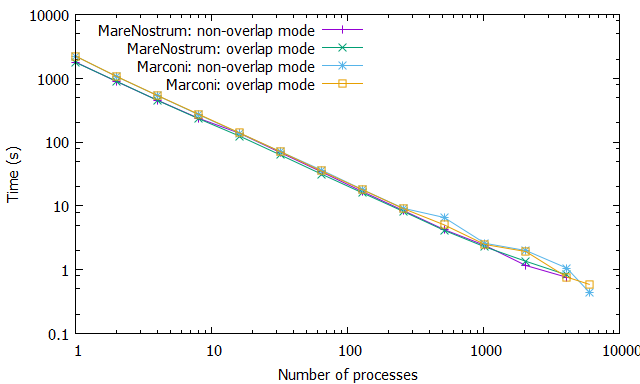
\includegraphics[width=0.8\textwidth]{FIGS/exaMD_strong_scaling_plot.png}
	\caption{Time to solution for runs of 32,000,000 particles in a $400^3$ domain with a cut-off radius of 8.0 on MareNostrum and Marconi.}
	\label{FIG_strong}
\end{figure}

Figure~\ref{FIG_weak} shows weak scaling performance on the same two machines, where both the number of particles and the size of the box are scaled with the core count. There are 15,625 particles per core and a box size of $50\times 25 \times 25$ per core. The cut-off distance was always 8.0. One dimension of the box is doubled with each doubling of the core count, so at two cores the box size will be $50\times 50 \times 25$, at four cores it will be $50\times 50 \times 50$ and at eight cores it will be $100\times 50 \times 50$. This means that for the biggest runs at 4,096 cores, the particle count was 64 million and the box size was $800\times 400 \times 400$. Each point is the mean of five runs.
\begin{figure}
	\centering
	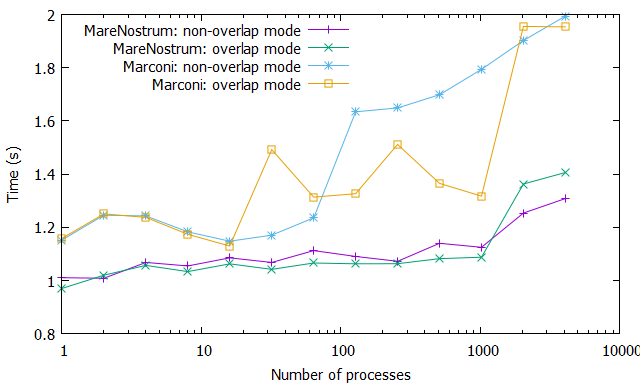
\includegraphics[width=0.8\textwidth]{FIGS/exaMD_weak_scaling_plot.png}
	\caption{Time to solution for weak-scaling runs on MareNostrum and Marconi.}
	\label{FIG_weak}
\end{figure}

The results show that MareNostrum consistently performs the better of the two machines. Its scaling graphs are also smoother. Comparing the overlap variant with the standard method on either machine, it is not possible to draw any conclusions about one method being better. Both the strong and the weak scaling graphs show good scaling up to the largest jobs run. Having said that, a comparison with a non-midpoint method is required in order to draw any conclusions about whether and in what circumstances it would be a better approach. Hopefully, this proto-app would allow someone to make such a comparison for their particular problems. 

%%%%%%%%%%%%%%%%%%%%%%%%%%%%%%%%%%%%%%%%%%%%%%%%%%%%%%%%%%%%%%%%%%%%%%%%%%%%%%%%%%%%%%%%%%%%%%%%%%%%%%%%%%%%%%%%%%%%%%%%%%%%%%%%%%%%%%%%%%%%%%%%%%%%

\begin{thebibliography}{1}
\bibitem{Larson08}
{R.H. Larson, J.K. Salmon, R.O. Dror, M.M. Deneroff, C. Young,
                      J.P. Grossman, Y. Shan, J.L. Klepeis, and D.E. Shaw.
`High-Throughput Pairwise Point Interactions in Anton,
a Specialized Machine for Molecular Dynamics Simulation'
IEEE 14th International Symposium on High Performance Computer Architecture.  (2008)}

\bibitem{Bowers06}
{ K.J. Bowers, E. Chow, Huageng Xu, R.O. Dror, M.P. Eastwood, B.A. Gregersen, J.L. Klepeis, I. Kolossvary, M.A. Moraes, F.D. Sacerdoti, J.K. Salmon, 
Yibing Shan and D.E. Shaw. 
`Scalable Algorithms for Molecular Dynamics Simulations on Commodity Clusters'
Supercomputing 2006, Proceedings of the ACM/IEEE.  (2006)}

\bibitem{FSSM17}
{ F. Sterpone and S. Melchionna.
`Adaptive Midpoint method for parallel Molecular Dynamics'
in preparation.}

\bibitem{Karypis06}
{A. Abou-Rjeili and G. Karypis. `Multilevel Algorithms for Partitioning Power-Law Graphs.'    
IEEE International Parallel \& Distributed Processing Symposium (IPDPS), (2006).}
        
\bibitem{Karypis02}
{K. Schloegel, G. Karypis, and V. Kumar.  `Parallel static and dynamic multi-constraint graph partitioning.'
\textsl{Concurrency and Computation: Practice and Experience} \textbf{14}:3 pp 219--240.  (2002)}
        
\end{thebibliography}                      

\end{document}
